% Los colores morado y celeste est�n definidos en la cabecera del archivo principal
%\def\fondoportada{\vbox to 0pt{\vspace*{-4.35cm}\hspace*{-4.61cm}
%\begin{tikzpicture}
%\shade[upper left=black, upper right=morado,
%lower left=morado, lower right=celeste] (0,0) rectangle (\paperwidth,\paperheight);
%\end{tikzpicture}\vss}}
\definecolor{rojodebil}{rgb}{0.82, 0.58, 0.6}
\def\fondoportada{\vbox to 0pt{\vspace*{-4.35cm}\hspace*{-4.61cm}
\begin{tikzpicture}
\shade[upper left=black, upper right=morado,
lower left=morado, lower right=rojodebil] (0,0) rectangle (\paperwidth,\paperheight);
\end{tikzpicture}\vss}}

% Nombre del bolet�n, N�mero XX, mes a�o
\long\def\cabeceraboletin{\noindent
{\color{white}
\hspace*{-.12\linewidth}\begin{tabular}{r}
\resizebox{1.2\textwidth}{!}{\resizebox{!}{3cm}{\calligra B}\resizebox{!}{1.6cm}{\calligra olet�n}
\resizebox{!}{.8cm}{ \textbf{electr�nico de la} }\resizebox{!}{1cm}{\textbf{SEMA}}} \\[2em]
\resizebox{!}{.7cm}{\textbf{\Numeromesanyo}} \\[3em]% N�mero XX, mes a�o
\end{tabular}}}

% Nombre del bolet�n, N�mero XX, mes a�o
\long\def\cabecerasobreindice{\noindent
{\color{azulsema}%
\resizebox{\textwidth}{!}{\resizebox{!}{3cm}{\calligra B}\resizebox{!}{1.6cm}{\calligra olet�n}
\resizebox{!}{.8cm}{ \textbf{electr�nico de la} }\resizebox{!}{1cm}{\textbf{SEMA}}}

\vspace*{.6cm}

\mbox{}\noindent\resizebox{!}{.5cm}{%
   \color{azulsema!60!black}\textbf{\Numeromesanyo}}% N�mero XX, mes a�o
}\vspace*{.6cm}}


\def\Numeromesanyo{N�mero 25, octubre 2020}
\pagestyle{myheadings}
\markboth{~\hrulefill\ Bolet�n electr�nico de la SEMA. \Numeromesanyo}{Bolet�n electr�nico de la SEMA. \Numeromesanyo\ \hrulefill\ }

\SinTikZ

\thispagestyle{empty}
\fondoportada
\vspace*{-2cm}

\cabeceraboletin


%\vspace*{1.5cm}
\vspace*{3.25cm}

% La foto:
\noindent\hspace*{-0.055\linewidth}\vbox to 0pt{%
%\includegraphics[width=1.1\linewidth]{portada-cedya2020.pdf}
\qquad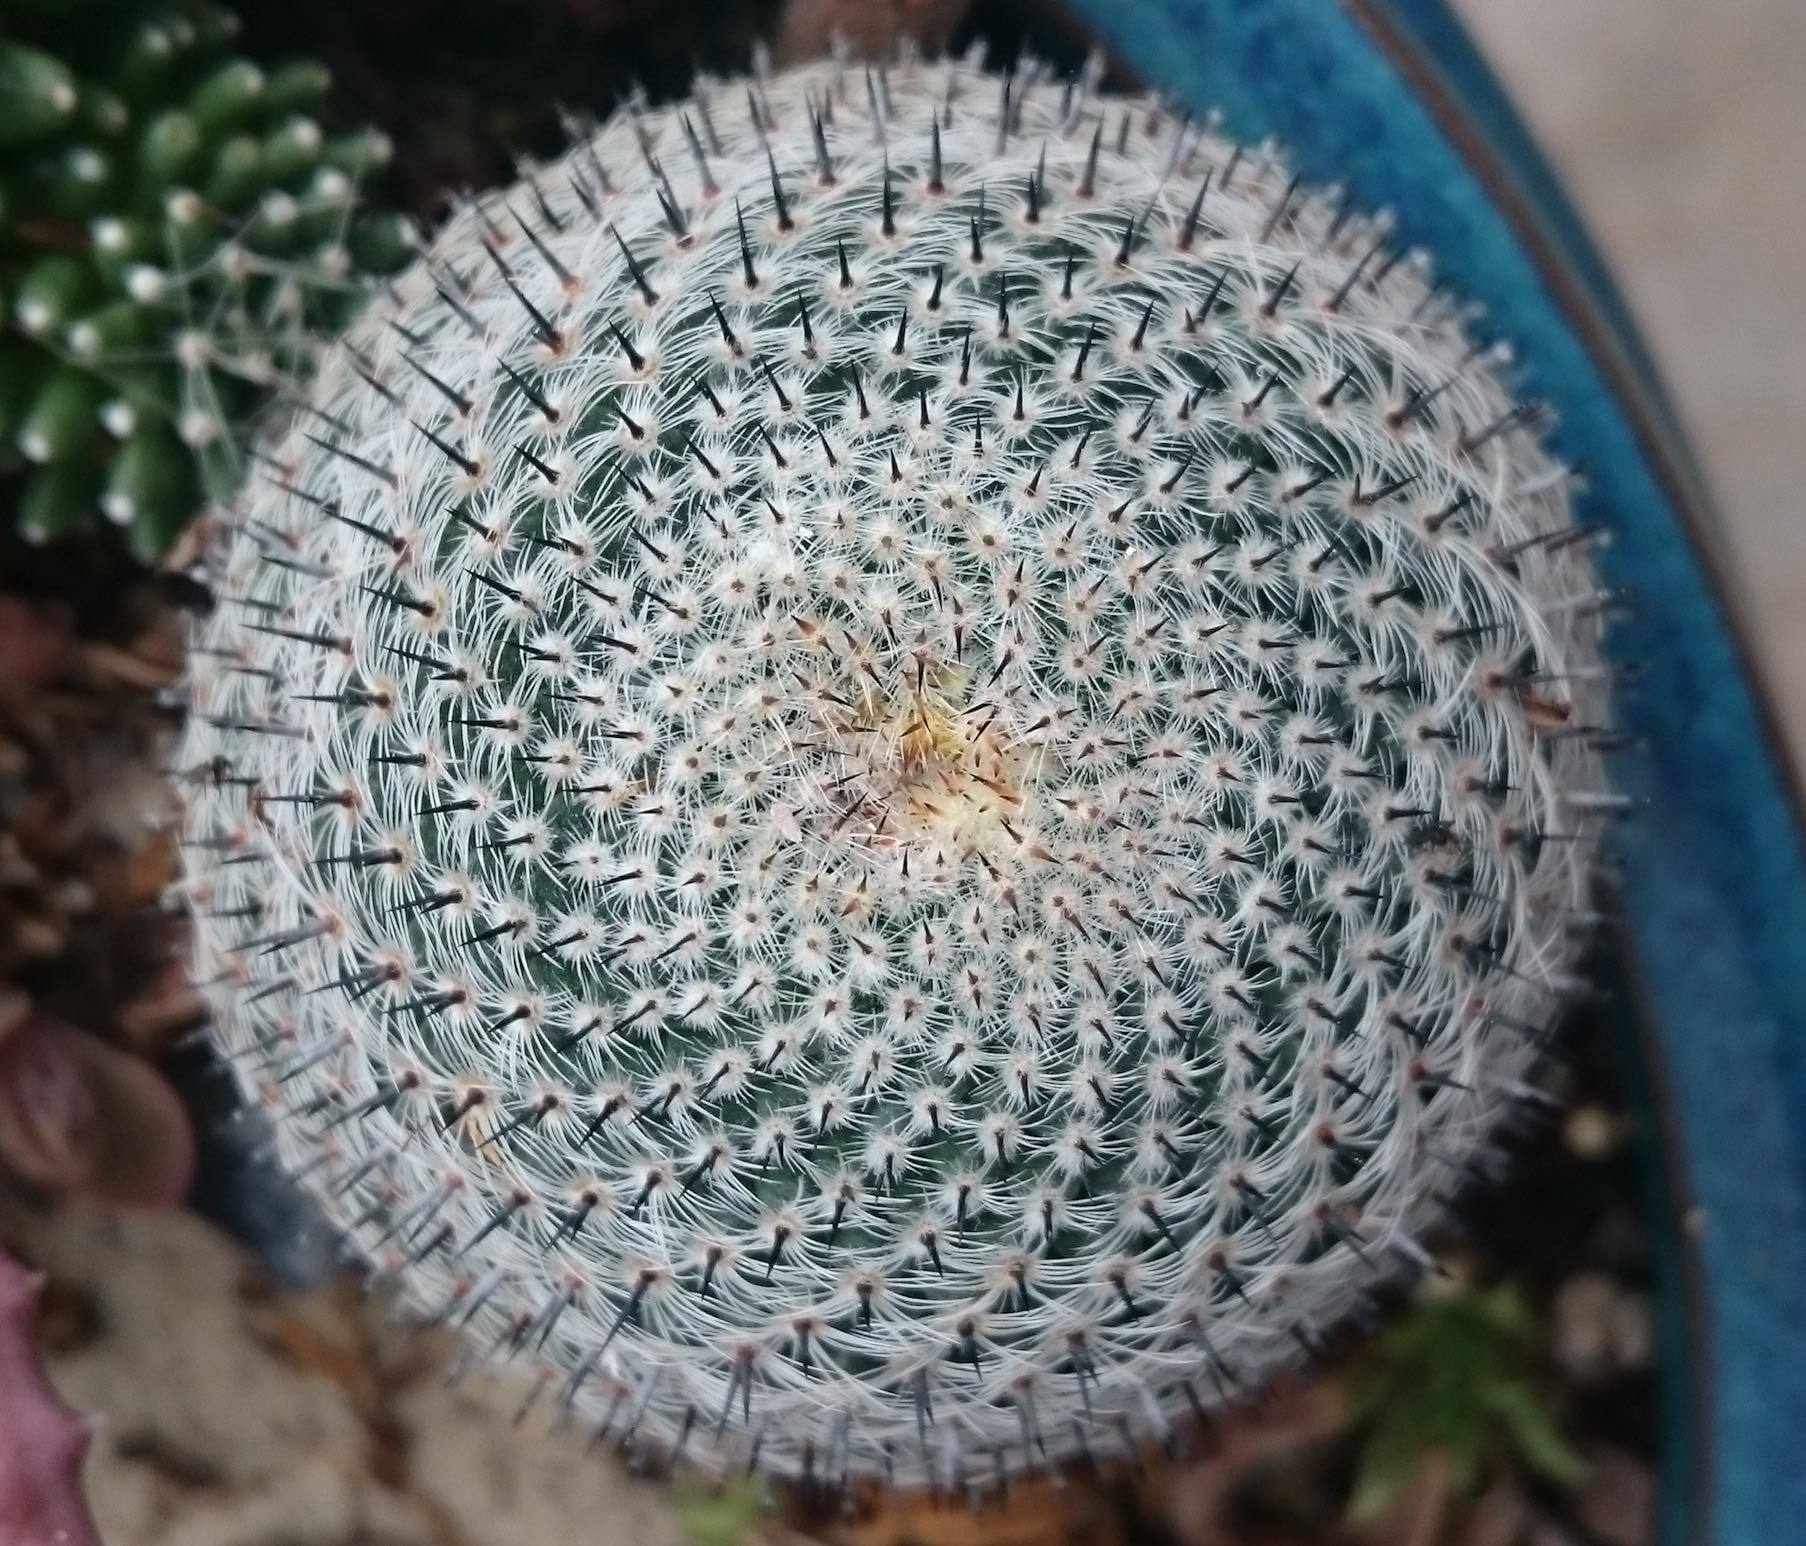
\includegraphics[width=1\linewidth]{cactus.jpg}
\vspace{-10.95cm}
\par\hspace{5ex}
%\resizebox{\linewidth}{1.67em}{\color{white!50!yellow}A un a�o del ICIAM2019, Valencia 15-19 julio 2019}
}

\vfill

%\def\nodeshadowed[#1]#2;{%
% \node[scale=2,  #1, yscale=1.1, scope fading=north, opacity=0.9, xshift=1pt, yshift=.6pt, xslant=0.1]{\global\setbox116=\hbox{#2}\copy116};
%  \node[scale=2,  #1]{{\color{white}\box116}};}
%
%\noindent\vbox to 1em{\vbox to 5em{\vss\resizebox{\linewidth}{3.5em}{\begin{tikzpicture}
%\nodeshadowed [at={(0,0)}] {\textbf{Sociedad Espa�ola de Matem�tica Aplicada}};
%\end{tikzpicture}}}} %Fin de la portada

\FinSinTikZ

\noindent\vbox to 1em{\vbox to 14em{\vss
\begin{center}
\hspace*{-0.085\linewidth}\includegraphics[width=1.2\linewidth]{../Identidad-corporativa-SEMA/PNG/300ppi/LOGO_SeMA_Mesadetrabajo1copia6.png}
\end{center}}}

%\noindent\vbox to 1em{\vbox to 5em{\vss\resizebox{\linewidth}{1.8em}{\color{white}\textbf{Sociedad Espa�ola de Matem�tica Aplicada}}}}


\newpage% p�gina detr�s de la portada
\thispagestyle{empty}
\mbox{}
\vspace{2cm}

\begin{tabular}{l@{\,}l}
& Bolet�n electr�nico de la SEMA -- \Numeromesanyo \\[1ex]
 & ISSN  2659-4129 \\[1cm]
\copyright & Sociedad Espa�ola de Matem�tica Aplicada -- SEMA\\[1ex]
\copyright & De los autores\\[1.5cm]
  &\includegraphics[width=.7\textwidth]{../Identidad-corporativa-SEMA/PNG/300ppi/LOGO_SeMA_Mesa-de-trabajo-4.pdf}\\[6ex]
  &{\large\url{https://www.sema.org.es/}}
\end{tabular}
\vfill

\noindent \textsl{Dise�o de la portada}: FOG.
\par\noindent
%\textsl{Imagen: Organizaci�n XXVI~CEDYA/CMA, Gij�n~2020.}
\textsl{Imagen: Esp�cimen de cactus mammillaria, donde son f�cilmente identificables sus exquisitas espirales �ureas. Foto: FOG.}
